% Created 2021-09-12 Sun 22:48
% Intended LaTeX compiler: xelatex
\documentclass[letterpaper]{article}
\usepackage{graphicx}
\usepackage{grffile}
\usepackage{longtable}
\usepackage{wrapfig}
\usepackage{rotating}
\usepackage[normalem]{ulem}
\usepackage{amsmath}
\usepackage{textcomp}
\usepackage{amssymb}
\usepackage{capt-of}
\usepackage{hyperref}
\usepackage[margin=1in]{geometry}
\usepackage{fontspec}
\usepackage{indentfirst}
\setmainfont[ItalicFont = LiberationSans-Italic, BoldFont = LiberationSans-Bold, BoldItalicFont = LiberationSans-BoldItalic]{LiberationSans}
\newfontfamily\NHLight[ItalicFont = LiberationSansNarrow-Italic, BoldFont       = LiberationSansNarrow-Bold, BoldItalicFont = LiberationSansNarrow-BoldItalic]{LiberationSansNarrow}
\newcommand\textrmlf[1]{{\NHLight#1}}
\newcommand\textitlf[1]{{\NHLight\itshape#1}}
\let\textbflf\textrm
\newcommand\textulf[1]{{\NHLight\bfseries#1}}
\newcommand\textuitlf[1]{{\NHLight\bfseries\itshape#1}}
\usepackage{fancyhdr}
\pagestyle{fancy}
\usepackage{titlesec}
\usepackage{titling}
\makeatletter
\lhead{\textbf{\@title}}
\makeatother
\rhead{\textrmlf{Compiled} \today}
\lfoot{\theauthor\ \textbullet \ \textbf{2021-2022}}
\cfoot{}
\rfoot{\textrmlf{Page} \thepage}
\titleformat{\section} {\Large} {\textrmlf{\thesection} {|}} {0.3em} {\textbf}
\titleformat{\subsection} {\large} {\textrmlf{\thesubsection} {|}} {0.2em} {\textbf}
\titleformat{\subsubsection} {\large} {\textrmlf{\thesubsubsection} {|}} {0.1em} {\textbf}
\setlength{\parskip}{0.45em}
\renewcommand\maketitle{}
\author{Houjun Liu}
\date{\today}
\title{RNA Replication}
\hypersetup{
 pdfauthor={Houjun Liu},
 pdftitle={RNA Replication},
 pdfkeywords={},
 pdfsubject={},
 pdfcreator={Emacs 28.0.50 (Org mode 9.4.4)}, 
 pdflang={English}}
\begin{document}

\maketitle


\section{RNA Replication}
\label{sec:org0b45727}
\subsection{The Strands of RNA}
\label{sec:org1016de8}
\begin{itemize}
\item +Strand: reproducable RNA => could be directly translated by the
ribosomes
\item -Strand RNA: useless template RNA (less easy to be detected)

\begin{itemize}
\item Need to be processed by RDRP (RNA-dependent RNA Polymerease)
\item Once entered the cell, RDRP goes to work copying -Strand RNA to
+Strang RNA
\end{itemize}

\item double-stranded RNA viron => (+, a.k.a. sense)

\begin{itemize}
\item +-stranded RNA => same idea as above

\item \begin{itemize}
\item strand RNA => virus comes with RDRP that convert -ssRNA to +ssRNA.
Then, same idea as above.
\end{itemize}
\end{itemize}
\end{itemize}

RNA-Dependent RNA polymerease catalyze this process of RNA replication.

\subsection{And\ldots{} Viruses!}
\label{sec:org621593c}
Because of the fact that the body will usually not need to create RNA
from only RNA, this mechnism is usually used by viruses to make more
copies of itself within a cell.

\begin{itemize}
\item RNA viruses does not need host-cell polymeraese to copy RNA
\item They come with polymerase that\ldots{}

\begin{itemize}
\item with dsRNA; takes +ssRNA and makes -ssRMA; combining the two to
produce dsRNA
\item with +ssRNA, takes +ssRNA and makes temporary -ssRNA which makes
more +ssRNA
\item with -ssRNA, takes -ssRNA, and makes temporary +ssRNA, which makes
-ssRNA
\end{itemize}
\end{itemize}

\begin{figure}[htbp]
\centering
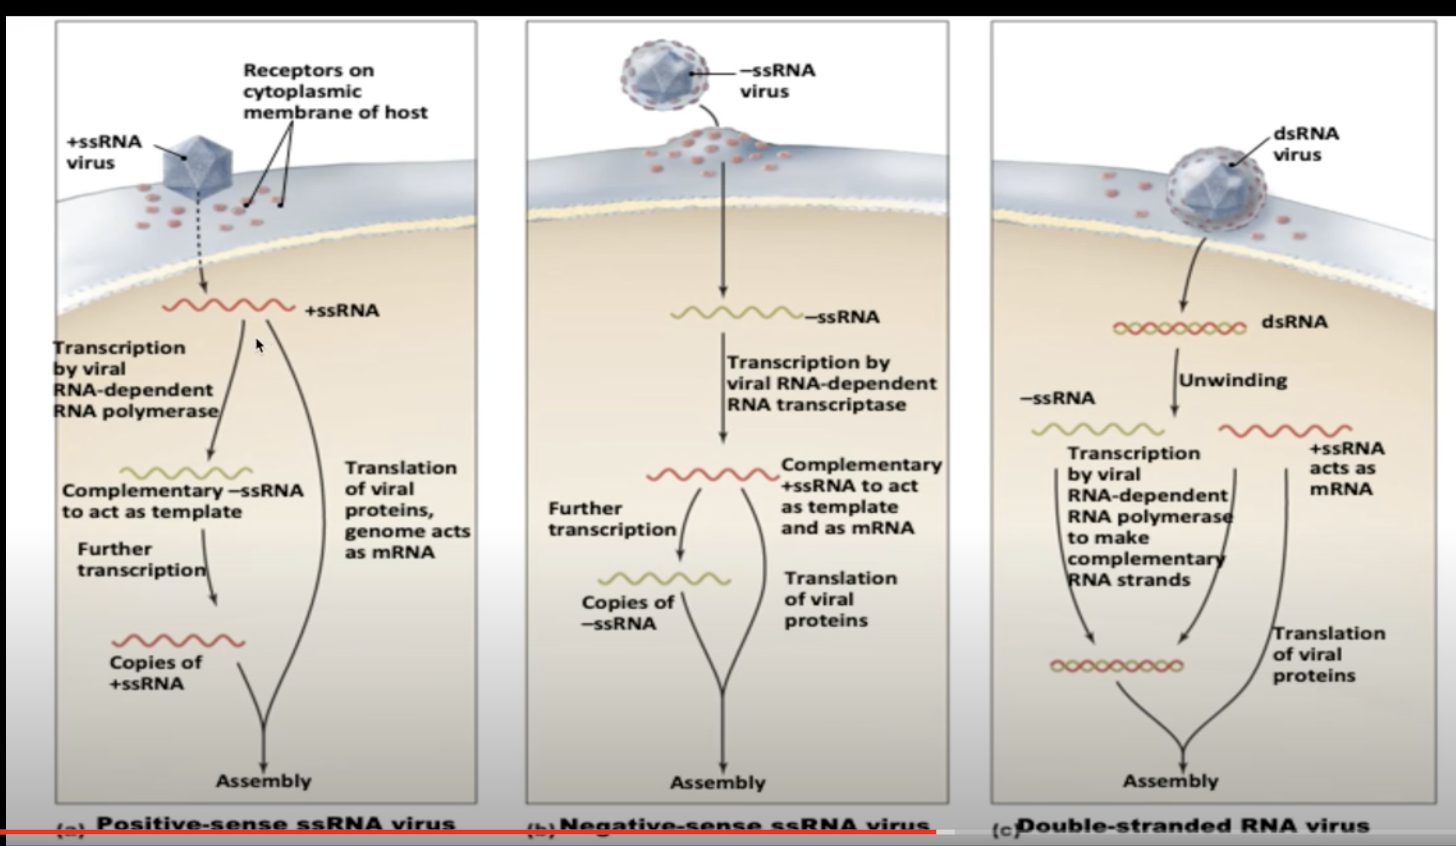
\includegraphics[width=.9\linewidth]{Screen Shot 2020-10-12 at 11.14.30 PM.png}
\caption{Screen Shot 2020-10-12 at 11.14.30 PM.png}
\end{figure}
\end{document}
